\Chapter{A TikZ és eszközkészlete}

\Section{Ábrák szerkesztése LaTeX-ben}

A rajzolás megkönnyítése érdekében a TikZ-t használjuk, amely egy frontend réteg a PGF-hez. Egy ábrát létrehozni azt jelenti, hogy egyenes vagy görbe vonalak sorozatát rajzoljuk meg. A TikZ parancsaira és szintaxisára olyan források voltak hatással, mint a METAFONT, a PSTricks és még sokan mások.

A pontokat és koordinátákat a TikZ egy speciális szintaxissal adja meg. A legegyszerűbb, ha kerek zárójelben vesszővel elválasztott két dimenziót használunk, például (4pt, 6pt). Ha az egység nincs megadva, akkor az xy-koordináta rendszerének alapértelmezett értékeit használjuk. Ez azt jelenti, hogy az egységnyi x-vektor 1 cm-rel jobbra, az egységnyi y-vektor pedig 1 cm-rel felfelé halad. 

\Section{A TikZ elemei}

\SubSection{Használata}

Először is be kell állítanunk a környezetünket. Ehhez a következőképpen néz ki a fájlunk:

\begin{lstlisting}[style=latex]
\documentclass{article}
\usepackage{tikz}
\begin{document}
    <content>
\end{document}
\end{lstlisting}

Ezután kezdhetjük el az ábrák létrehozását. 


\SubSection{Szintaxis}

A szabály az, hogy minden TikZ grafikus rajzoló parancsnak a \textit{tikz} parancs argumentumaként vagy a \textit{tikzpicture} környezeten belül kell előfordulnia. A környezeten belül megadott összes opció a teljes képre vonatkozik.

A \textit{tikzpicture} környezet \LaTeX\ változata a következő:

\begin{lstlisting}[style=latex]
\begin{tikzpicture}[options]
    <content>
\end{tikzpicture}
\end{lstlisting}


A TikZ-ben minden ábra alapvető építőeleme a vonal. Egy vonalat a kezdőpont koordinátáinak megadásával kezdünk, mint például (0,0), majd hozzáadunk egy vonal bővítő műveletet, erre a legkézenfekvőbb módszer csak a "\textit{- -}" használata. A műveletet ezután a következő koordináta követi. Minden útvonalnak pontosvesszővel kell végződnie. Az vonal megrajzolásához a \textit{draw} parancsot használjuk.

Például a (0,0), (0,1), (1,0)  pontok közötti háromszög felrajzolásához (egyik lehetséges módjaként) az alábbi parancsokat kell alkalmazni:

\begin{lstlisting}[style=latex]
\tikz\draw (0,0) -- (0,1) -- (1,0) -- (0,0);
\end{lstlisting}

vagy

\begin{lstlisting}[style=latex]
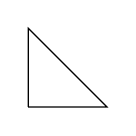
\begin{tikzpicture}
    \draw (0,0) -- (0,1) -- (1,0) -- (0,0);
\end{tikzpicture}
\end{lstlisting}

\begin{tikzcode}
\draw (0,0) -- (0,1) -- (1,0) -- (0,0);
\end{tikzcode}

\SubSection{Elérhető diagram elemek}

A körök és ellipszisek rajzolásához a \textit{circle} és \textit{ellipse} műveletet használhatjuk. A kör műveletet egy sugár követi kerek zárójelben, míg az ellipszis műveletet kettő paraméter követi, egy az x-irányra és egy az y-irányra vonatkozóan, amelyeket az \textit{and} taggal választunk el, és kerek zárójelben helyezünk el. 

\begin{tikzcode}
\draw (0,0) circle (1);
\end{tikzcode}

\begin{tikzcode}
\draw (0,0) ellipse (1 and 0.5);
\end{tikzcode}

\begin{tikzcode}
\draw (0,0) ellipse (0.5 and 1);
\end{tikzcode}

A rácsháló (\textit{grid}), téglalap (\textit{rectangle}), a parabola (\textit{parabola}), és az ív (\textit{arc}) rajzolásához további, a korábbiakhoz hasonlóan működő műveletek állnak rendelkezésünkre. Az alábbiak példák ezen konstrukciók használatára:

\begin{tikzcode}
\draw (-1,-1) grid (1,1);
\end{tikzcode}

\begin{tikzcode}
\draw (-1,0) -- (1,0);
\draw (0,-1) -- (0,1);
\draw (0,0) circle (1);
\draw (-1,-1) rectangle (1,1);
\draw (-1,-1) parabola (1,1);
\end{tikzcode}

Az ív használható például egy szög ívének megrajzolásához. Megrajzolja a kör adott sugarú részét a megadott szögek között. Ezt a műveletet egy kerek zárójelben lévő hármasnak kell követnie. Az adattagokat kettőspontok választják el egymástól. Az első és a második a kör fokai, a harmadik pedig a sugara. 

Például a (\textit{30 : 160 : 2cm}) azt jelenti, hogy egy 2 cm sugarú körön 30 és 100 fok közötti ív lesz:

\begin{tikzcode}
\draw (0,0) arc (30:100:2cm);
\end{tikzcode}

Az elemek elforgatásához vagy skálázásához egy \textit{rotate} vagy \textit{scale} opciót is hozzáadhatunk:

\begin{tikzcode}
\draw[rotate=45] 
	(0,0) ellipse (1 and 0.5);
\end{tikzcode}

\begin{tikzcode}
\draw[scale=1.5] 
	(0,0) ellipse (1 and 0.5);
\end{tikzcode}

Természetesen használhatjuk a két opciót együttesen is az alábbi szerint:

\begin{tikzcode}
\draw[rotate=45, scale=1.5] 
	(0,0) ellipse (1 and 0.5);
\end{tikzcode}

A \textit{color} csomagot hozzáadva a \textit{definecolor} paranccsal definiálhatunk és használhatunk színeket az alábbiak szerint:
\begin{tikzcode}
\definecolor{myRGB}{RGB}{255, 51, 76}
\definecolor{myrgb}{rgb}{1, 0.2, 0.3}
\definecolor{mycmyk}{cmyk}{0, 0.8, 0.7, 0}
\definecolor{mygray}{gray}{0.3}

\draw [myRGB] (0,1) -- (1,1);
\draw [myrgb] (0,0.5) -- (1,0.5);
\draw [mycmyk] (0,0) -- (1,0);
\draw [mygray] (0,-0.5) -- (1,-0.5);
\end{tikzcode}

Az általunk definiált színeknek négyféle megadási módja lehetséges:

\begin{itemize}
	\item[] \textit{RGB}: a szabványos RGB-modell szerinti megadással megegyezik: a három színkomponens a piros (\textit{R}), zöld (\textit{G}), és a kék (\textit{B}), melyek értéke $[0,255]$ közötti egész számok.
	\item[] \textit{rgb}: a fenti \textit{RGB}-modell $[0,1]$ közötti normalizált értékei. 
	\item[]  \textit{cmyk}: cián (\textit{c}), magenta (\textit{m}), sárga (\textit{y}) és fekete (\textit{k}), mely négy [0,1] közötti, vesszővel elválasztott, számból álló lista, amelyek a kereskedelmi nyomtatók által használt szubtraktív CMYK-modell szerint határozzák meg a színt.
	\item[] \textit{gray}: ez egy szürke skála, melynek megadása egyetlen szám, ami $[0,1]$ közötti.
\end{itemize}

A következő színeket érhetjük el bármiféle definiálás nélkül: 

\begin{table}[!htbp]
	\centering
	\renewcommand{\arraystretch}{0}
	\addtolength{\tabcolsep}{-4pt}
	\begin{tabular}{@{}llllllllllll@{}}
	\textit{white} & (\tikz\draw (0,0) rectangle (0.5,0.25);), & 
	\textit{lightgray} & (\tikz\fill [lightgray](0,0) rectangle (0.5,0.25);), &
	\textit{gray} & (\tikz\fill [gray](0,0) rectangle (0.5,0.25);), & 
	\textit{darkgray}& (\tikz\fill [darkgray](0,0) rectangle (0.5,0.25);), & 
	\textit{black}& (\tikz\fill [black](0,0) rectangle (0.5,0.25);), & 
	\textit{red}& (\tikz\fill [red](0,0) rectangle (0.5,0.25);), \\
	
	\textit{violet}& (\tikz\fill [violet](0,0) rectangle (0.5,0.25);), &
	\textit{purple}& (\tikz\fill [purple](0,0) rectangle (0.5,0.25);), &
	\textit{magenta}& (\tikz\fill [magenta](0,0) rectangle (0.5,0.25);), &
	\textit{pink} &(\tikz\fill [pink](0,0) rectangle (0.5,0.25);), &
	\textit{green} &(\tikz\fill [green](0,0) rectangle (0.5,0.25);), &
	\textit{lime} &(\tikz\fill [lime](0,0) rectangle (0.5,0.25);), \\
	
	\textit{olive} &(\tikz\fill [olive](0,0) rectangle (0.5,0.25);), &
	\textit{brown} &(\tikz\fill [brown](0,0) rectangle (0.5,0.25);), &
	\textit{orange}& (\tikz\fill [orange](0,0) rectangle (0.5,0.25);), &
	\textit{yellow}& (\tikz\fill [yellow](0,0) rectangle (0.5,0.25);), &
	\textit{blue} &(\tikz\fill [blue](0,0) rectangle (0.5,0.25);), &
	\textit{cyan}& (\tikz\fill [cyan](0,0) rectangle (0.5,0.25);), \\
	
	\textit{teal} &(\tikz\fill [teal](0,0) rectangle (0.5,0.25);). &
	\end{tabular}
\end{table}

A \textit{fill} paranccsal kitölthetjük a megadott színnel a bármely alakzat által határolt tartományt. Az aktuális rajzolt görbe lezárásához használhatjuk a \lstinline[style=latex]{-- cycle} parancsot. A szín argumentumhoz használhatjuk a szín nevét, például \textit{green} (\tikz\fill [green](0,0) rectangle (0.5,0.25);), \textit{white} (\tikz\draw (0,0) rectangle (0.5,0.25);) és \textit{red} (\tikz\fill [red](0,0) rectangle (0.5,0.25);), vagy keverhetjük a színeket, mint a \textit{red!40!white}, ami azt jelenti, hogy 40\% pirosat és 60\% fehéret fogunk keverni.

\begin{tikzcode}
\fill[red!40!white] 
	(0,0) -- (0,1) -- (1,0) -- cycle;
\end{tikzcode}

A kitöltést meg lehet adni egyszerűen a \textit{draw} parancs paramétereként is, ám ilyenkor a körvonal is rajzolva lesz:

\begin{tikzcode}
\draw[fill=red!40!white] 
	(0,0) -- (0,1) -- (1,0) -- cycle;
\end{tikzcode}

Ez a színmegadás természetesen használható a körvonal színének módosítására is:

\begin{tikzcode}
\draw[draw=green, fill=red!40!white] 
	(0,0) -- (0,1) -- (1,0) -- cycle;
\end{tikzcode}

A vonalakat végpontjait testreszabhatjuk, így nyilakat hozhatunk létre:

\begin{tikzcode}
\draw [->] (0,1) -- (1,1);
\draw [<-] (0,0.5) -- (1,0.5);
\draw [|-|] (0,0) -- (1,0);
\end{tikzcode}

A nyílhegyek esetében is rengeteg lehetséges opció van, a két végponton lévő nyílhegy szabadon variálható. Egy pár ezek közül:
\begin{tikzcode}
\draw [stealth-stealth reversed] (0,1.5) -- (1,1.5);
\draw [to-to reversed] (0,1) -- (1,1);
\draw [latex-latex reversed] (0,0.5) -- (1,0.5);
\draw [|-|] (0,0) -- (1,0);
\end{tikzcode}

Az \textit{arrows.meta} könxvtár további nyílhegyeket tartalmaz, ebből két darabot emelnék ki, melyek jól használhatók a fentiekkel kombinálva:

\begin{tikzcode}
\draw [{Stealth[open]}-stealth reversed] (0,0.5) -- (1,0.5);
\draw [{Latex[open]}-latex reversed] (0,0) -- (1,0);
\end{tikzcode}

Ha több szegmenst rajzolunk, a nyilak az első és az utolsó szegmens végpontjainál helyezkednek el. Ez, többek között, a tengelyek rajzolásához kényelmes:

\begin{tikzcode}
\draw [<->] (0,1) -- (0,0) -- (1,0);
\end{tikzcode}

Az attribútumokkal a vonalvastagságok módosítására is van lehetőség:

\begin{tikzcode}
\draw [thin] (0,1) -- (1,1);
\draw [thick] (0,0.5) -- (1,0.5);	
\draw [ultra thick] (0,0) -- (1,0);
\end{tikzcode}

Azonban ügyelni kell rá, hogy a vonal vastagsággal arányosan nő a nyíl mérete is:

\begin{tikzcode}
\draw [->, thin] (0,1) -- (1,1);
\draw [->, thick] (0,0.5) -- (1,0.5);	
\draw [->, ultra thick] (0,0) -- (1,0);
\end{tikzcode}

A vonal stílusának módosítására is van mód, a jelentős számú lehetőség közül az alábbiakat emelném ki:

\begin{tikzcode}
\draw [dotted] (0,1) -- (1,1);
\draw [dashed] (0,0.5) -- (1,0.5);	
\draw [dashdotted] (0,0) -- (1,0);
\end{tikzcode}

A pontok és szaggatott vonalak sűrűsége a \textit{loosely} (lazán) és a \textit{densely} (sűrűn) jelzővel adható meg.
\begin{tikzcode}
\draw [dashed] (0,1) -- (1,1);
\draw [loosely dashed] (0,0.5) -- (1,0.5);	
\draw [densely dashed] (0,0) -- (1,0);
\end{tikzcode}

Az eddigi testreszabással kapcsolatos paraméterek akár együttesen is szerepelhetnek:

\begin{tikzcode}
\draw [|-latex, red, thick, dashed] (0,0) -- (1,0);
\end{tikzcode}

Ahhoz, hogy szöveget adjunk a képhez, csomópontot kell hozzáadnunk az útvonalhoz, mint a következőben:

\begin{tikzcode}
\draw 
    (1,1) node[circle,draw]{A} 
        -- 
    (2,2) node[circle,draw]{B};	
\end{tikzcode}

A csomópontok az útvonal aktuális pozíciójába kerülnek, a [\textit{circle,draw}] opció a szöveget egy körrel veszi körül, amely az aktuális pozícióba rajzolódik.

Adott esetben szükség lehet rá, ha a csomópont az aktuális koordináta jobb oldalán vagy fölött lenne. Ehhez viszont már szükséges a \textit{positioning} könyvtár hozzáadása is a fájlunkhoz az alábbi szerint:

\begin{lstlisting}[style=latex]
\usetikzlibrary{positioning}
\end{lstlisting}

\begin{tikzcode}
\draw 
(1,1) node[anchor=north east, circle, draw]{A} 
	-- 
(2,2) node[anchor=south west, circle, draw]{B}; 
\end{tikzcode}

A csomópont stílusok egyenként tetszés szerint módosíthatóak. Ezekre szintén attribútumokat használunk:

\begin{tikzcode}
\draw (0,2) node[circle, draw]{Circle};



\draw (0,0) node[rectangle, draw]{Rectangle}; 
\end{tikzcode}


\Section{Szerkesztőeszközök}

A következőkben a már meglévő, és népszerű szerkesztőkörnyezetek kerülnek bemutatásra, valamint kifejtésre kerülnek az összehasonlító szempontok, amik kritériumok lesznek a készülő alkalmazás felé.

\SubSection{draw.io}

A kezelőfelület fejlécében az általános menüpontok szerepelnek. Az alkalmazás közepén van maga a felület, ahol az ábrák szerkeszthetők. Ezt fogja körbe a bal oldalról az ábrákkal kapcsolatos, míg jobb oldalon a diagram beállításai, és előre definiált stílusok közül lehet választani. 

Az alapelemek csoportosítva vannak kinézetük alapján lenyitható menüpontokként. 

\begin{figure}[!h]
	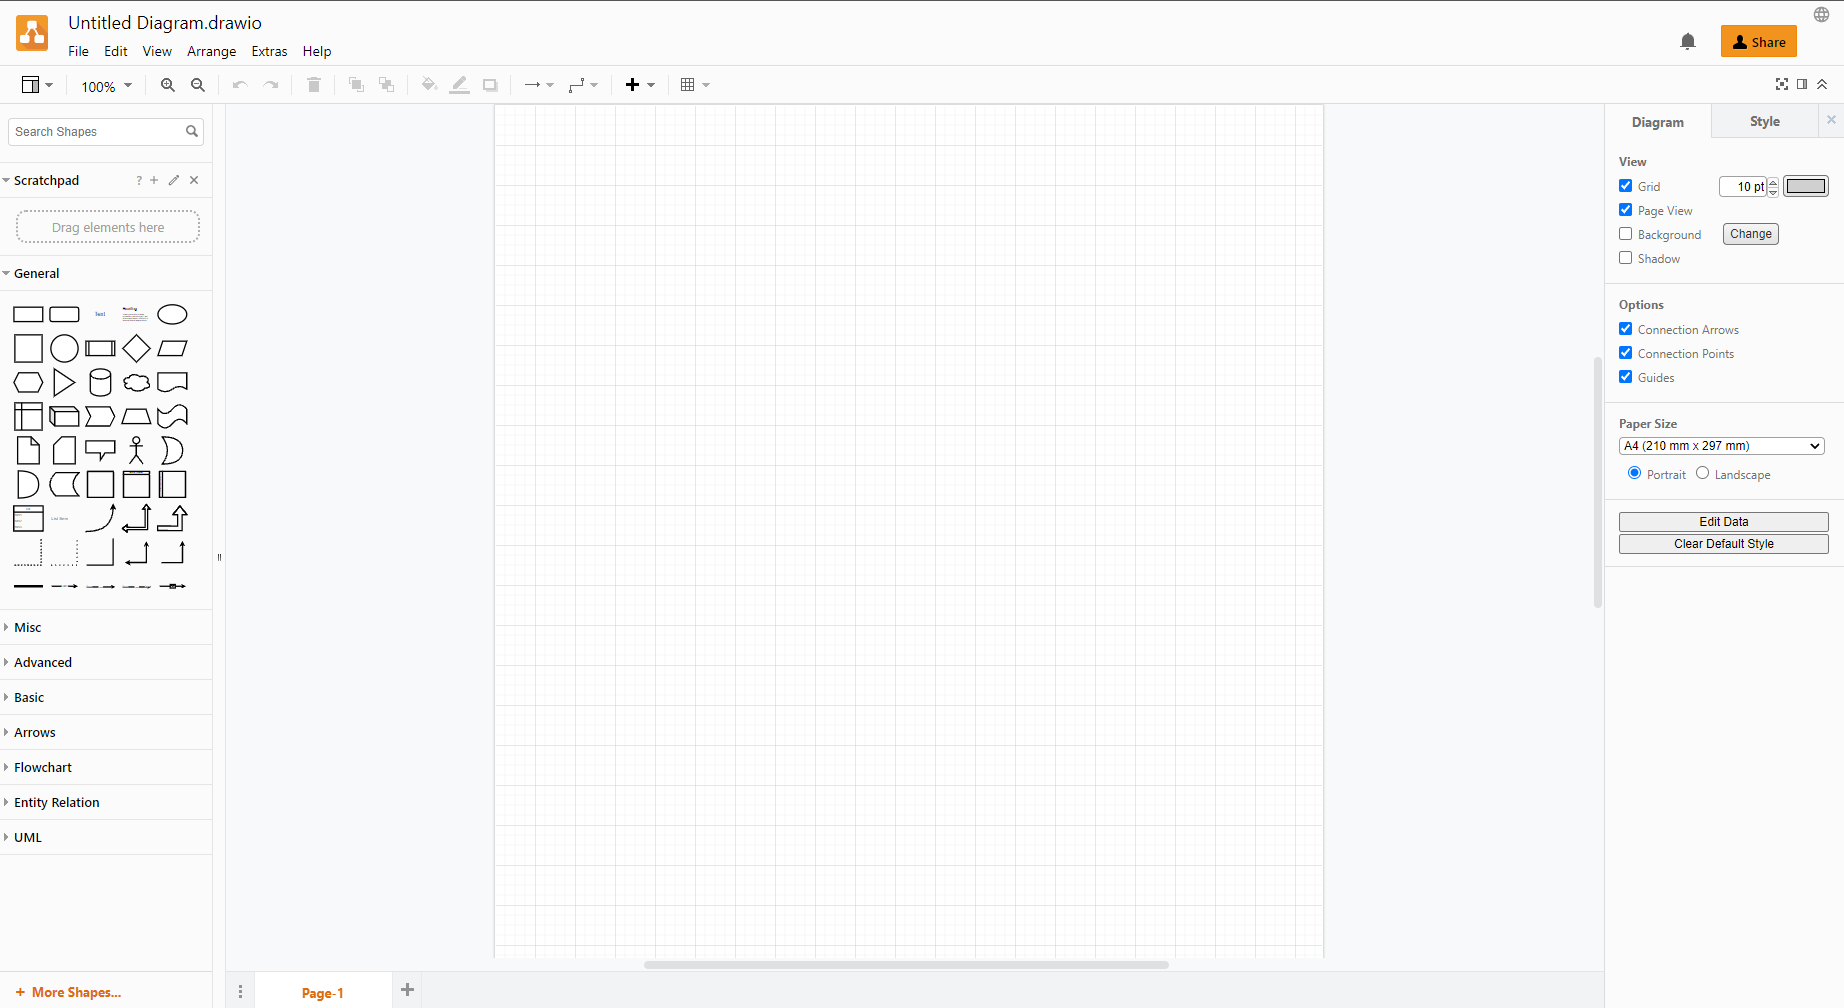
\includegraphics[width=\textwidth]{images/drawio.png}
	\caption{A draw.io kezelőfelülete \cite{drawio}}
	\label{fig:drawio}
\end{figure}

Az ábra kiválasztása után rögtön megjelenik a felület közepén, ezt követően lehet elhelyezni. Az ábrák szerkesztésénél több lehetőség áll rendelkezésünkre. Az előre definiált pár stíluson felül többféleképpen is meg lehet adni saját színeket is: RGB színválasztóval, hexakódokkal, és gyakran használt színekkel egyaránt. Be lehet állítani az adott ábrára kitöltőszínt, betűszínt, vízszintes és függőleges igazítást, árnyékot, bemetszést.

Bármelyik ábrára helyezhető szöveg, ennek a stílusa igazodik az alakzat stílusához. Az objektumok bárhol összekapcsolhatók, de megjelennek ajánlott pontok is: 0, 25, 50, 75 és 100\%-on. A rétegek nem jelennek meg külön oldalon, az ábrák sorrendje számít, hogy melyik jelenik meg felül. A kijelölés téglalap alapú, a kijelölt elemeket lehet másolni, törölni, szerkeszteni. Az ábrák csak rácspontokhoz igazíthatók.

Az alkalmazás rendelkezik Undo-Redo funkciókkal. 

Az elkészített diagram menthető különböző fájlformátumokban, automatikusan mentésre kerülnek a módosítások. 


\SubSection{TikZiT}

A TikZiT leginkább gráfok rajzolására használható. A vezérlő elemek az alkalmazás fejlécében helyezkednek el. A grafikus alapelemek szintén itt találhatóak, számuk nem kiemelkedő: a kijelölésen kívül van egy gráf csomópont lerakásához és egy gráf éleinek berajzolásához egy gomb. 

Mind a csomópont, mind a gráf stílusa módosítható, fájlként menthető, és betölthető, a programon belül és kívül is (a kód ismeretében) szerkeszthetők. Három lehetőség van: alak, szín, kitöltés. 

\begin{figure}[!h]
	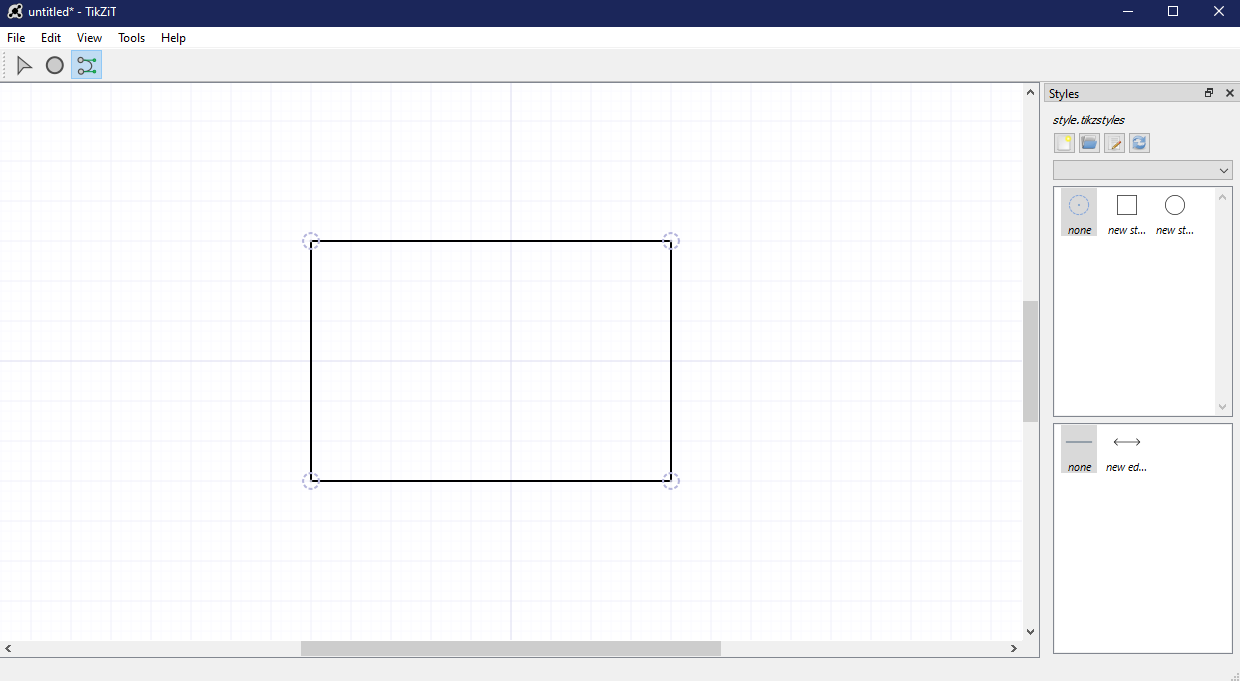
\includegraphics[width=\textwidth]{images/tikzit.png}
	\caption{A TikZiT kezelőfelülete \cite{tikzit}}
	\label{fig:tikzit}
\end{figure}

A szín és kitöltés kiválasztása történhet előre definiált alapszínekből, de lehetőség van RGB színskálából kiválasztásra vagy hexakód megadására is. Szöveg a gráf csomópontjainak adható. A csomópontokat összekötő élek a két pont helyzetétől függenek, csak az él hajlítására van lehetőség. 

A csomópontok rétegződését a lerakás sorrendje határozza meg, utólag csak kijelölés után van lehetőség előre vagy hátra küldeni az adott elemet. A kijelölés téglalap alakú, a kijelölt elemek másolhatók, törölhetők, stílusuk szerkeszthető.  

A program rendelkezik Undo-Redo funkciókkal, a rajzolófelületen lehetőség van nagyításra és kicsinyítésre egyaránt. 

A kész ábrák mentése fájlba történik, ezek betölthetők későbbi szerkesztésre is, automatikus mentés nincs.

\SubSection{TikzEdt}

\begin{figure}[!h]
	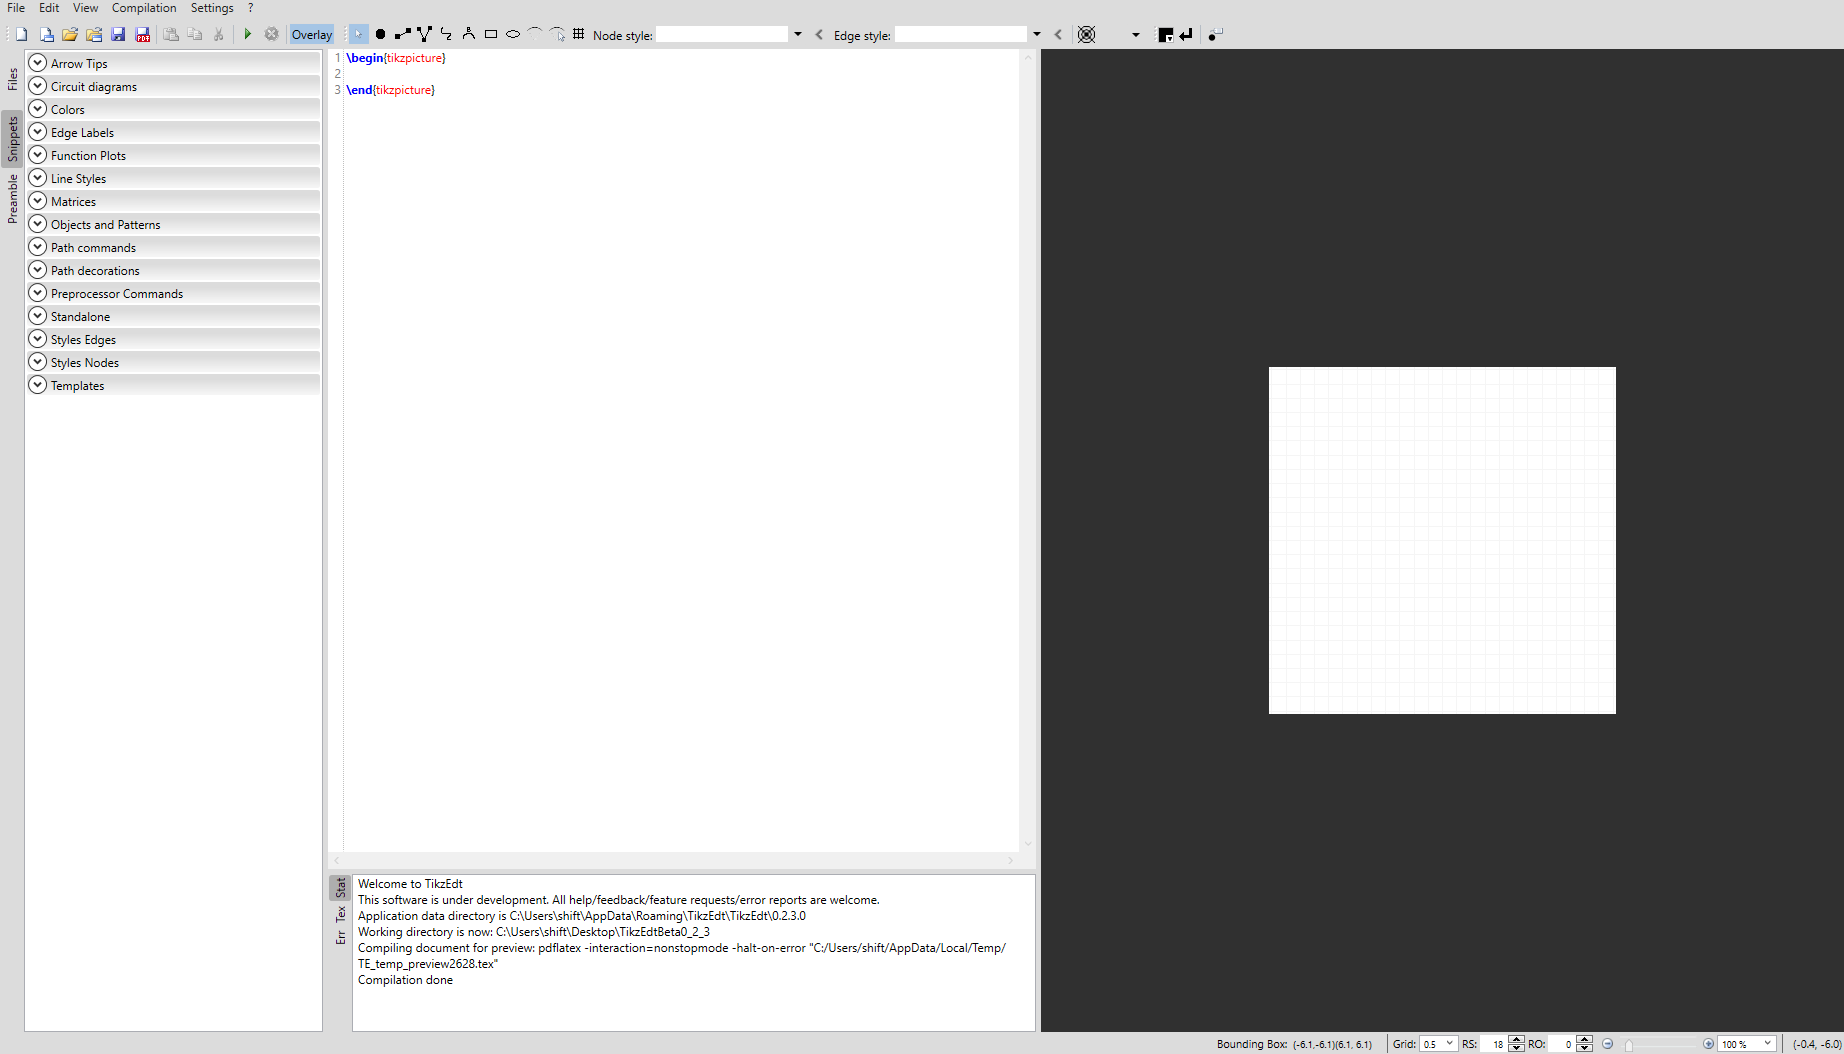
\includegraphics[width=\textwidth]{images/tikzedt.png}
	\caption{A TikzEdt kezelőfelülete \cite{tikzedt}}
\label{fig:tikzedt}
\end{figure}

A TikzEdt esetében három hasábra osztható a felület: elsőben az előre definiált \LaTeX\ kódrészletek, másodikban a LaTeX kódszerkesztő, és végül a harmadikban a lefordított kód előnézete jelenik meg. 

Az alapelemek a felső sávban jelennek meg: főleg gráfokkal és egyszerűbb elemeket tartalmaz. Az elemek, gráfok, egyenletek, szövegek stílusa és színei csak kód szinten szerkeszthetők, de vannak választható opciók. 

A rétegződés a lerakás sorrendjében jön létre, utólagos módosításra nincs lehetőség. Az elemek automatikusan rácspontokhoz igazodnak. 

A kijelölés téglalap alakú, a kijelölt elemek csak törölhetők. A program rendelkezik Undo-Redo funkciókkal, a rajzolófelületen lehetőség van nagyításra és kicsinyítésre egyaránt. 

A kész ábrák mentése fájlba történik, automatikus mentés nincs.

\SubSection{tikzcd-editor}

A \textit{tikzcd-editor} klasszikus felülettel nem rendelkezik, csak egy négyzet alapú rácsháló fogad megnyitáskor. A rácsok közepére igazítva lehet nyilakat rajzolni, és szövegeket írni, de utólag van lehetőség a fel-le mozgatásra. 

A stílusok nem testreszabhatók, csak pár alap stílusból lehet választani, mint a szaggatott vagy dupla vonal, módosítható a nyíl eleje, illetve vége. A rácsokon belül gombnyomásra tudunk hurkot rajzolni. A nyilakra és vonalakra kifejezések rakhatók. Az elemek színei nem módosíthatók, ezen a felületen kizárólag fekete vonalszínnel lehet dolgozni.

A rétegződés a lerakás sorrendjében van. Az elemek kijelölése csak egyesével működik, nincs lehetőség téglalap vagy esetleg lasszó alapú kijelölésre. A kijelölt rács a felületen szabadon mozgatható, és áthelyezhető üres cellákba.

A szerkesztő rendelkezik Undo-Redo funkciókkal, de mentésre nincs lehetőség, csak a \LaTeX\ kód kimásolására, és az ábrához tartozó link utólagos betöltésére.

Az alkalmazás felépítését megnézve a felület egy felsorolás, aminek a stílusa erőteljesen testre lett szabva, hogy a rácsháló kinézetet megkapja. A rácsok szerkesztésével igazából a felsorolás pontjai kerülnek módosításra.

\begin{figure}[!h]
	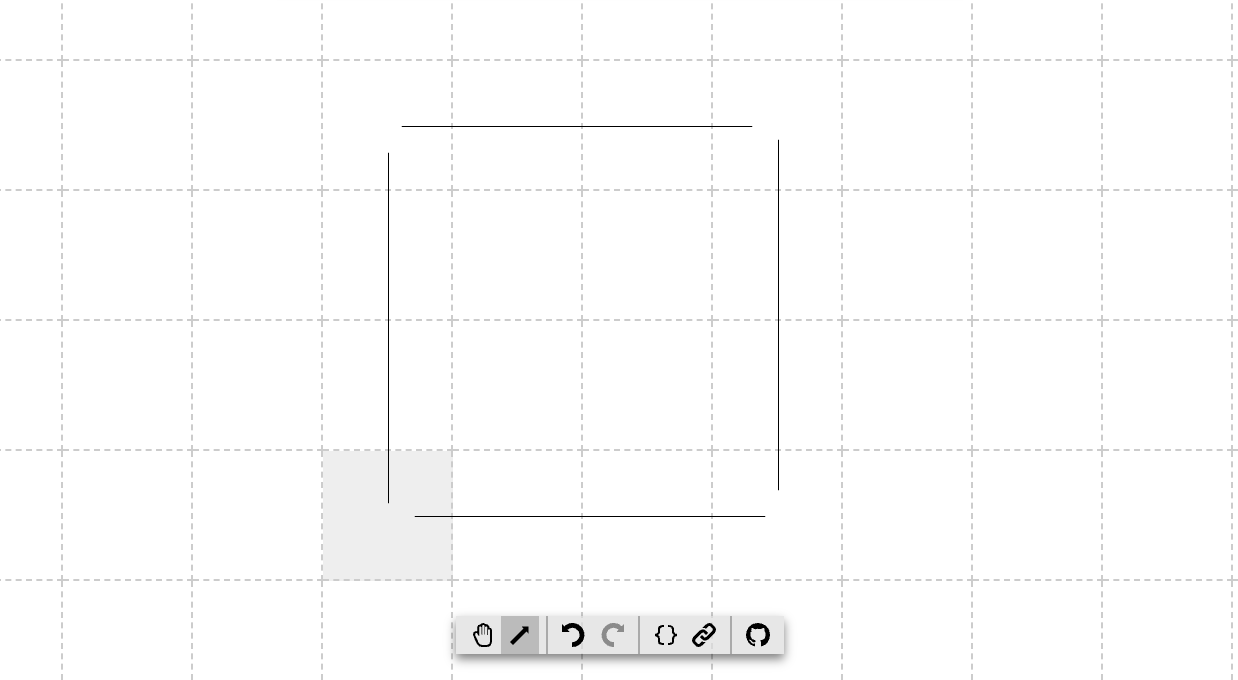
\includegraphics[width=\textwidth]{images/tikzcd.png}
	\caption{tikzcd-editor kezelőfelülete \cite{tikzcd}}
	\label{fig:tikzcd}
\end{figure}


\SubSection{Összehasonlítás}

Szempontok, amik alapján az összehasonlítást végzem:

\begin{description}
	\item[Elrendezés:] Az elrendezés az, amivel a szerkesztő megnyitásakor a felhasználó először találkozik. Fontos, hogy átlátható, és egyszerűen kezelhető legyen. A leggyakoribb alkalmazás elrendezések közül kettőt emelnék ki: egyik az fejléc és maga a szerkesztőfelület, a másik a hasáb alapú felépítés, ahol az alkalmazás részei egymás mellett jelennek meg. 
	\item[Alapelemek megjelenítése:] Az alapelemek helyzete is épp ilyen fontos, a felhasználó szempontjából kifejezetten előnyös, ha Megfelelő (logikus) szempontok alapján csoportosítva vannak az alapelemek, és nem csak egymás után fel vannak sorolva, akár egy mátrix alapú felépítésben.
	\item[Tulajdonságok szerkesztése:] Ha már leraktunk egy objektumot, akkor elvárható az, hogy a lent lévő elem szerkeszthető is legyen: ez érinti a helyzetet, színeket, és a stílusokat is. Itt szükséges lehetőséget adni a szerkesztendő elemek kiválasztására, akár magán a rajzolófelületen, akár egy listában kijelölve.
	\item[Szövegek szerkesztése:] Elérhetővé kell tenni a felhasználó számára a szövegek szerkesztését: szabadon, vagy a csomópontokon belüli megjelenítést. Ebben az esetben is kiválaszthatónak kell lennie a szerkesztendő szövegeknek.
	\item[Színek megadási módja:] Az ábrák színezhetők, így a szerkesztőnek is tudni kell kezelni a színeket: legalább az előre definiált színeket kiválaszthatóvá kell tenni.
	\item[Objektumok összekapcsolási módja:] A már kész objektumokat milyen módon lehet összekötni: előre definiált fix helyeken, az körvonalain bárhol, vagy egyáltalán nincs lehetőség összekapcsolásra. 
	\item[Objektumok automatikus igazítása:] Rendelkezik-e a szerkesztő olyan funkcióval, amely az objektum pontjait automatikusan a vászon bizonyos pontjaira illeszti, és ez az opció esetleg be- és kikapcsolható.
	\item[Rétegek kezelése:] Van-e lehetőség rétegek létrehozására, vagy sem, az elemek sorrendje a mérvadó, vagy van lehetőség utólag rendezni az objektumokat. 
	\item[Kijelölés:] Milyen formában van lehetőség objektumok kijelölésére: téglalap, lasszó, kattintás alapú kijelölés vagy egyáltalán nincs lehetőség objektumok kijelölésére. Téglalap és lasszó alapú kijelölés esetén egyszerre több elem is kijelölhető, még a kattintás alapú kijelölés esetén egy kattintással csak egy elem jelölhető ki, esetleg funkciógombokkal (mint például a \textit{CTRL}, vagy az \textit{ALT} billentyű) van lehetőség több elemet kijelölni.
	\item[Másolás és beillesztés:] A kijelölt objektumot van-e lehetőség másolni valamilyen formában a vászonra: vezérlőgombok a szerkesztőben vagy az alkalmazások között népszerűnek számító \textit{CTRL + C} és \textit{CTRL + V} billentyűkombinációk elérhetők az alkalmazáson belül.
	\item[Zoom-olás:] A vászont lehet-e valamilyen formában nagyítani a precízebb rajzolás miatt vagy esetleg kicsinyíteni a nagyobb rajzolási felület érdekében. 
	\item[Undo-Redo funciók:] Az alakzat rajzolásának vagy módosításának visszavonására van-e lehetőség. A véletlenül visszavont szerkesztések megismétlésére milyen lehetőségek állnak rendelkezésre. A könnyű elérés miatt célszerű ezeket is billentyűkombinációkra rakni: \textit{CTRL + Z} és \textit{CTRL + Y} billentyűkombinációk.
	\item[Automatikus mentés:] A szerkesztő menti-e a rajzolás közben a munkamenetet, vagy teljes mértékben a felhasználóra van bízva a mentés folyamata.
\end{description}

\begin{table}[]
	\caption{Szerkesztőeszközök összefoglalása az előző szempontok szerint}
	\label{tab:editors}
	\medspace
	
	\centering
	\begin{tabular}{|l|c|c|c|c|}
		\hline
		& draw.io & tikzit & tikzedt& tikzcd\\ \hline
		
		Elrendezés  & \multicolumn{3}{c|}{hasáb felépítés} & alul\\ \hline
		
		\begin{tabular}[c]{@{}l@{}}Alapelemek \\ megjelenítése\end{tabular}& \begin{tabular}[c]{@{}c@{}}mátrix alapú, \\ csoportosítva\end{tabular} & sorban & \begin{tabular}[c]{@{}c@{}}lenyíló listás \\ rendezés\end{tabular} & sorban \\ \hline
		
		\begin{tabular}[c]{@{}l@{}}Tulajdonságok \\ szerkesztése\end{tabular} & \multicolumn{2}{c|}{előre definiált stílusok}& \begin{tabular}[c]{@{}c@{}}csak kód \\ szinten\end{tabular} & \begin{tabular}[c]{@{}c@{}}kijelölés \\ után\end{tabular} \\ \hline
		
		\begin{tabular}[c]{@{}l@{}}Szövegek \\ szerkesztése\end{tabular}& bárhol & \multicolumn{2}{c|}{csak csomópontokon} &  \begin{tabular}[c]{@{}c@{}}rácsok \\ közepén\end{tabular} \\ \hline
		
		\begin{tabular}[c]{@{}l@{}}Színek megadási \\ módjai\end{tabular}& \multicolumn{2}{c|}{\begin{tabular}[c]{@{}c@{}}előre definiált színek, \\ RGB, és HEX  megadás\end{tabular}} & \begin{tabular}[c]{@{}c@{}}csak kód \\ szinten\end{tabular}& nem \\ \hline
		
		
		\begin{tabular}[c]{@{}l@{}}Objektumok\\ összekapcsolási\\ módjai\end{tabular} & bárhol & \multicolumn{2}{c|}{középen} & nem \\ \hline
		
		\begin{tabular}[c]{@{}l@{}}Objektumok\\ automatikus \\ igazítása\end{tabular} & igen & \multicolumn{2}{c|}{nem} & igen \\ \hline
		
		Rétegek kezelése & \multicolumn{4}{c|}{rajzolási sorrend} \\ \hline
		
		Kijelölés & téglalap alapú & \multicolumn{3}{c|}{kattintás alapú} \\ \hline
		
		\begin{tabular}[c]{@{}l@{}}Másolás és \\ beillesztés\end{tabular} & \multicolumn{2}{c|}{igen} & \begin{tabular}[c]{@{}c@{}}csak kód \\ szinten\end{tabular} & nem \\ \hline
		
		Zoom-olás & \multicolumn{3}{c|}{igen} & nem \\ \hline
		
		\begin{tabular}[c]{@{}l@{}}Undo-redo \\ funkciók\end{tabular} & \multicolumn{4}{c|}{igen} \\ \hline
		
		\begin{tabular}[c]{@{}l@{}}Automatikus \\ mentés\end{tabular} & igen & \multicolumn{3}{c|}{nem} \\ \hline
	\end{tabular}
\end{table}

